%!TeX root = ProgramaciónEvolutiva.tex
\section*{Evolutionary computing}
\begin{frame}
  \begin{blur}
    \begin{center}
      {\LARGE Evolutionary programming}
    \end{center}
  \end{blur}
\end{frame}

\begin{frame}
  \begin{blur}

    Following what John R. Koza said in his essay Human-Competitive Machine
    Intelligence \cite{PEADNAS2003}, points that evolutionary algorithms can be
    used in order to make a computer program to solve (approximately)
    a problem.

  \end{blur}
\end{frame}

\begin{frame}[fragile,allowframebreaks]{The problem, the model and the solution}
  \begin{blur}

  Think about a problem. Usually, to solve some problem, we can solve it
  using tools that are already available. For example, if we want to know
  the position of a particle at a certain time in an uniform rectilinear
  motion problem, we can solve it by a simple equation.
  \begin{figure}[!ht]
    \begin{center}
    \begin{tikzpicture}[>=Stealth, font=\sffamily\small]

      % Experiment surface
      \draw[thick, fill=black!90] (0,0) rectangle (8,1);
      \draw[<->] (0,-0.5) -- (8,-0.5) node[right]{$X$};

      %Equation $X_f(t) = X_0 + V_0 t$
      \draw node at (4,1.8) {$X_f(t) = X_0 + V_0 t$};

      % Moving object
      \filldraw[fill=blue!30, draw=blue!50!black] (1,0.5) rectangle node[black]{$m$} (2,1.2);

      % Force arrow
      \draw[->, Yellow, thick] (2,0.85) -- node[above]{$\vec{V}$} (3.5,0.85);

      % Measurement markers
      \foreach \x in {0,2,4,6,8} {
        \draw (\x,0) -- (\x,-0.15) node[below]{$\x$};
      }

    %% Motion trace
    %\draw[decorate, decoration={snake, amplitude=0.5mm, segment length=2mm}] 
    %(2,1.4) -- node[above]{Motion trace} (6,1.4);

    % Coordinate axes
    %\draw[->] (0.2,0.2) -- (0.2,1.2) node[right]{$y$};
    %\draw[->] (0.2,0.2) -- (1.2,0.2) node[above]{$x$};

    \end{tikzpicture}
    \end{center}
    \caption{Uniform rectilinear motion [Deepseek]}
  \end{figure}

  \end{blur}
  \begin{blur}
    And we can call it a simulation, which is the most common thing, and
    easiest thing to do with a computer.
  \end{blur}
  
  \begin{beamerlst}[language=python]
class Particle:
  def __init__(self, x0, v0):
    self.x0 = x0
    self.v0 = v0

  def simulate(self, t):
    return self.x0 + self.v0 * t

  def __repr__(self):
    return f'Particle(x0={self.x0}, v0={self.v0})'
     
if __name__ == '__main__':
  p = Particle(0, 10)
  print(p.simulate(10))
  \end{beamerlst}
  \begin{center} \rule{0.9\linewidth}{0.4pt} \end{center}

  \vfill

  \begin{beamerlst}
  %% Output as in a python shell
  >_ python particle.py
  100
  \end{beamerlst}

  \vfill

  \begin{center} \rule{0.9\linewidth}{0.4pt} \end{center}
  \newpage

  \begin{blur}
    But now, what happens if we haven't an equation or an algorithm to solve
    the problem? If have data and we need to know how it's behaving? What if
    we need to predict it's behaviour? Maybe some nonlinear phenomena,
    a signal, classification, or something not so intuitive as common
    problems? 
  \end{blur}
  
  \begin{blur}
    Here is where modeling comes in \cite{Eiben2015}. And here is where genetic programming
    started to gain relevance.
  \end{blur}
  

\end{frame}

\begin{frame}[allowframebreaks]{Modeling}

    \begin{blur}
      Genetic programming is an implementation of genetic algorithms where
      the individuals are programs which are intended to solve a given
      problem

      \begin{figure} [!ht]
        \begin{center}
          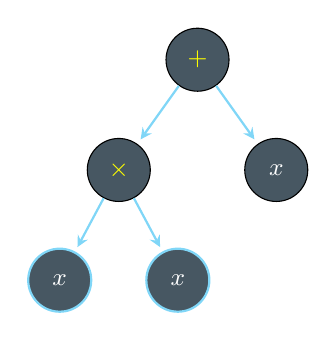
\begin{tikzpicture}[
            x=0.4cm, y=0.4cm,
            level distance=1.4cm,
            level 1/.style={sibling distance=2cm},
            level 2/.style={sibling distance=1.5cm},
            every node/.style={
              draw, 
              circle, 
              fill=cyan!30!black, 
              text=white, 
              minimum size=0.8cm,
              font=\small
            },
            edge from parent/.style={
              draw, 
              ->, 
              >=stealth, 
              shorten >=2pt, 
              thick, 
              cyan!50
            }
            ]

          % Root node (+)
            \node {\textcolor{Yellow}{$+$}}
            child {
                  % Left subtree (x^2)
              node {\textcolor{Yellow}{$\times$}}
              child {
                node {$x$}
              }
              child {
                node {$x$}
              }
            }
            child {
                  % Right subtree (x)
              node {$x$}
            }
            ;
          \end{tikzpicture}
        \end{center}
        \caption{Genetic programming solution tree for $x^2 + x$ [Deepseek]}
      \end{figure}
    \end{blur}


    \section{Ejemplos}
    \begin{blur}

      Aquí se muestra un ejemplo de la implementación de un algoritmo genético para
      programación genética utilizando el framework DEAP \cite{DEAPGENETIC}.

      \begin{itemize}
        \item \href{run:./Ejemplo/DEAP-GP.html} {\underline{Ejemplo HTML}}
        \item \href{run:./Ejemplo/DEAP-GP.pdf}   {\underline{Ejemplo PDF}}
        \item \href{run:./Ejemplo/DEAP-GP.ipynb}{\underline{Ejemplo Jupyter}}
        \item \href{run:./Ejemplo/DEAP_GP.py}   {\underline{Ejemplo Python}}
    \end{itemize}

    \end{blur}

\end{frame}
